\documentclass[11pt,a4paper]{article}
\usepackage[utf8]{inputenc}
\usepackage[T1]{fontenc}
\usepackage[margin=2.2cm]{geometry}
\usepackage{amsmath,amssymb}
\usepackage{booktabs}
\usepackage{graphicx}
\usepackage{xcolor}
\usepackage{hyperref}
\usepackage{caption}
\usepackage{subcaption}
\usepackage{microtype}
\usepackage{enumitem}

\hypersetup{
    colorlinks=true,
    linkcolor=blue!70!black,
    citecolor=blue!70!black,
    urlcolor=blue!70!black
}

\title{\textbf{Flight Arrival Efficiency, Fuel Penalties, and Machine Learning on European Air Traffic}\\[0.4em]
\large A Medallion PySpark Pipeline on EUROCONTROL OPDI Data}
\author{\textbf{Mathis Nancey} \quad \& \quad \textbf{Thomas Canisares--Morère}\\
\small Group 08 \quad | \quad Course: DAT535 Data Engineering\\
\small Department of Electrical Engineering and Computer Science, University of Stavanger (UiS)}
\date{Production Run: \texttt{prod-8} (2026-11-09) \quad | \quad Autumn Semester 2026}

\begin{document}

\maketitle

\begin{abstract}
This project implements an industrial-grade distributed data pipeline using \textbf{PySpark 3.5} following a Medallion architecture (Bronze, Silver, Gold, ML, Summary) to analyze \textbf{58 days} of open flight trajectory data from \textbf{EUROCONTROL OPDI v0.0.2} and aerodrome master records from \textbf{OurAirports} (June 1 -- July 28, 2026). The pipeline ingests and standardizes \textbf{3,304,717 flights}, \textbf{86,670,133 flight events}, and \textbf{118,779,222 physical trajectory measurements} (5.46~GB raw). We investigate flight arrival efficiency across five airports: Paris-CDG (\texttt{LFPG}), Toulouse-Blagnac (\texttt{LFBO}), and Stavanger Sola (\texttt{ENZV}), benchmarked against London-Heathrow (\texttt{EGLL}) and Frankfurt (\texttt{EDDF}). 

Empirical findings from production run \texttt{prod-8} show that \textbf{London-Heathrow} is severely constrained by runway throughput saturation, with 12.7\,\% of arrivals entering holding patterns (32,802 holding minutes) and average additional arrival time reaching 4.9~min. Conversely, \textbf{Paris-CDG} and \textbf{Frankfurt} exhibit low holding rates (2.9\,\%) but suffer from vertical descent inefficiencies, accumulating 4.6 and 4.1 minutes of intermediate level flight per arrival, resulting in estimated excess fuel burn of $\sim$30 and $\sim$34 tonnes/day under EUROCONTROL CDO benchmarks. \textbf{Toulouse} and \textbf{Stavanger} display near-optimal fluid descents (1.6 and 0.2 min of level flight). A Spark MLlib \texttt{GBTRegressor} predicts additional transit time with a test MAE of 2.74~min (beating the naive baseline of 2.84~min), revealing that aerodrome infrastructure accounts for 55.0\,\% of delay variance. A simulated 90th-percentile demand cap yields daily delay reductions of 7.0~min at Frankfurt and 6.8~min at Toulouse.
\end{abstract}

\section{Introduction and Operational Context}

Managing arrival air traffic in congested airspace requires balancing runway throughput, flight safety, and fuel efficiency. While cruise flight is largely optimized by modern Flight Management Systems (FMS), the descent and arrival phase is vulnerable to tactical air traffic control (ATC) interventions. When terminal airspace or runway capacity is saturated, controllers resort to two primary delay-absorption techniques:
\begin{enumerate}[noitemsep,topsep=2pt]
    \item \textbf{Airborne Holding Patterns (Holdings):} Racetrack-shaped orbits flown at assigned flight levels while awaiting landing slots.
    \item \textbf{Descent Level-Offs (Step-Downs):} Interrupting an optimal idle-thrust Continuous Descent Operation (CDO) with intermediate horizontal segments to maintain vertical aircraft separation.
\end{enumerate}

Both maneuvers incur heavy fuel and emission penalties: jet turbine engines operate with lower thermal efficiency at lower altitudes, where dense air increases aerodynamic drag. According to EUROCONTROL, flying level during descent consumes approximately \textbf{12.7~kg of kerosene per minute} (fleet average), emitting \textbf{3.16~kg of $\text{CO}_2$ per kg of fuel}.

\paragraph{Research Question:}
\textit{How much time and fuel do commercial flights lose before landing at Paris-CDG (\texttt{LFPG}), Toulouse-Blagnac (\texttt{LFBO}), and Stavanger (\texttt{ENZV}) --- benchmarked against London-Heathrow (\texttt{EGLL}) and Frankfurt (\texttt{EDDF}) --- when, why, and what operational interventions could mitigate these penalties?}

\paragraph{Methodological Boundary:}
The EUROCONTROL OPDI v0.0.2 open dataset does \textbf{not} contain scheduled airline timetable times. Consequently, this study adheres to EUROCONTROL Performance Review Unit (PRU) principles: delay is measured not as commercial schedule deviation, but as \textbf{additional transit time} relative to an empirical, unconstrained (20th-percentile) reference flight. Furthermore, findings represent statistical associations and operational factors, not causal claims, as atmospheric winds and convective weather are unobserved.

\section{Data Engineering Pipeline and Architecture}

The pipeline is implemented as a modular Python package (\texttt{projet\_opdi/src/opdi\_pipeline/}) managed via a unified CLI (\texttt{run\_pipeline.py}) and parameterized through TOML configurations (\texttt{dev.toml} for a 10-day sample, \texttt{prod.toml} for the 58-day scope).

\subsection{Medallion Architecture Overview}
The system transitions data across five functional layers:
\begin{itemize}[noitemsep,topsep=2pt]
    \item \textbf{Ingestion (\texttt{ingestion.py}):} Downloads 16 source files via HTTP with exponential backoff, records cryptographic SHA-256 digests in a persistent manifest, verifies disk safety quotas (\texttt{min\_free\_gb = 4.0}), and detects upstream file republications.
    \item \textbf{Bronze (\texttt{bronze.py}):} Stores source CSV data verbatim as partitioned Parquet tables. Injects row-level lineage metadata (\texttt{\_source\_file}, \texttt{\_source\_row\_num}, \texttt{\_ingest\_run\_id}, \texttt{\_bronze\_at\_utc}). Implements an \textbf{incremental state manager} (\texttt{\_state.json}) tracking SHA-256 hashes; unmodified partitions are skipped, reducing Bronze build time from 525.7~s in \texttt{prod-4} to \textbf{0.4~s} in \texttt{prod-8}.
    \item \textbf{Silver (\texttt{silver.py}, \texttt{arrivals.py}):} Cleanses timestamps, casts coordinates, harmonizes missing values, and enforces referential integrity. Implements a \textbf{Quarantine Engine} isolating anomalous rows (\texttt{quarantine\_flights}: 625 rows with duration $>24$h; \texttt{quarantine\_flight\_events}: 9,100 orphan events). Computes arrival indicators via 100~NM ring crossing interpolation, 200~NM descent profiles, and level-off fusion.
    \item \textbf{Gold (\texttt{gold.py}):} Executes declarative Spark SQL star-schema queries (\texttt{sql/*.sql}) to generate operational summaries (movements, runway allocations, ground times, arrival metrics, and holding hotspots). Enforces 30 automated validation checks before atomic publication with a \texttt{\_SUCCESS} marker.
    \item \textbf{Machine Learning (\texttt{ml.py}):} Trains a Spark MLlib \texttt{GBTRegressor} on complete-hour measured arrivals, evaluates feature importances, simulates demand-capping policies, and fits a \texttt{KMeans} airport typology ($k=3$).
    \item \textbf{Summary \& Quality Gates (\texttt{quality.py}):} Evaluates 7 strict, blocking quality gates guaranteeing zero-defect data promotion.
\end{itemize}

\begin{table}[t]
\centering
\small
\caption{Production Data Accounting (Run \texttt{prod-8}, 58 days).}
\label{tab:accounting}
\begin{tabular}{llr}
\toprule
\textbf{Layer} & \textbf{Table / Entity} & \textbf{Record Count} \\
\midrule
Raw & Ingested OPDI source files (5.46 GB) & 16 files \\
Bronze & \texttt{flight\_list} & 3,304,717 \\
Bronze & \texttt{flight\_events} & 86,670,133 \\
Bronze & \texttt{measurements} & 118,779,222 \\
Bronze & \texttt{airports} / \texttt{runways} & 86,350 / 48,412 \\
\midrule
Silver & \texttt{flights} (clean, deduplicated) & 3,127,830 \\
Silver & \texttt{flight\_events} (referential integrity) & 84,000,238 \\
Silver & \texttt{arrivals} (known destination) & 1,866,643 \\
Silver & \texttt{descent\_level\_offs} (fused segments) & 1,919,728 \\
Quarantine & \texttt{quarantine\_flights} / \texttt{flight\_events} & 625 / 9,100 \\
\midrule
Gold & European Movements (dep / arr) & 3,636,308 \\
Gold & \texttt{airport\_hourly\_ops} / \texttt{daily\_ops} & 474,130 / 43,397 \\
Gold & \texttt{arrival\_reference} & 3,046 \\
Gold & \texttt{airport\_arrival\_daily} / \texttt{hourly} & 41,334 / 381,863 \\
Gold & \texttt{holding\_hotspots} & 20,438 \\
Gold & \texttt{airport\_typology} (clustered airports) & 119 \\
\bottomrule
\end{tabular}
\end{table}

\subsection{Performance Engineering \& Incident Resolution}
The pipeline executes on an Ubuntu 22.04 VM with 4 vCPUs, 7.8~GB RAM, and 38~GB storage, utilizing PySpark 3.5 in local mode with 2~GB driver memory. The complete production deployment (\texttt{prod-8}) executed in \textbf{14~min 43~s}: Ingestion (36~s), Bronze (19~s), Silver (10~min 35~s), Gold (1~min 8~s), and ML (1~min 2~s).

\paragraph{The \texttt{prod-5} Out-of-Memory Incident:}
During run \texttt{prod-5}, the pipeline crashed after 13 minutes with \texttt{java.lang.OutOfMemoryError: GC overhead limit exceeded}. Root cause analysis revealed that \texttt{arrivals.py} accepted \textit{lazy DataFrames} from preceding Silver steps. Spark repeatedly re-evaluated the full upstream DAG over 86.6 million events and performed unpartitioned joins across all 118.8 million measurements, exhausting driver memory during shuffle spills.
The issue was resolved (PRs \#12 and \#13) by:
\begin{enumerate}[noitemsep,topsep=2pt]
    \item Decoupling materialization: reading directly from persisted Silver Parquet files.
    \item Early spatial pre-filtering: restricting events to a 300~NM radius around destination aerodromes.
    \item Direct joins restricted to \texttt{type = 'Distance flown (NM)'}, bypassing full measurement aggregations.
    \item Staging intermediate level-off Parquet tables to disk before joining.
\end{enumerate}
This optimization reduced the arrival calculation to \textbf{215.7~s} without memory pressure.

\section{Arrival Efficiency Methodology}

\subsection{Indicator A: Additional Arrival Transit Time}
Quantifies horizontal terminal sequencing delay within a \textbf{100~NM ($185.2\text{~km}$)} radius of the aerodrome:
\begin{itemize}[noitemsep,topsep=2pt]
    \item \textbf{Entry Point ($t_{\text{entry}}$):} Interpolated timestamp where the trajectory crosses the 100~NM boundary. Entry bearings are assigned to 8 cardinal sectors of 45$^\circ$ (\texttt{N, NE, E, SE, S, SW, W, NW}).
    \item \textbf{Touchdown ($t_{\text{touchdown}}$):} Earliest \texttt{entry-runway} event at the destination with altitude $\le \text{elevation} + 1,500\text{~ft}$.
    \item \textbf{Unimpeded Baseline ($T_{\text{ref}}$):} Empirical 20th percentile of transit duration ($t_{\text{touchdown}} - t_{\text{entry}}$) for cohorts defined by $(\text{airport}, \text{runway}, \text{aircraft\_class}, \text{entry\_sector})$, with hierarchical fallback cascades for small sample sizes ($N < 20$).
    \item \textbf{Additional Transit Time:} $\Delta t_{\text{arr}} = (t_{\text{touchdown}} - t_{\text{entry}}) - T_{\text{ref}}$, filtered to plausible transits between 5 and 120 minutes.
\end{itemize}

\subsection{Indicator B: Vertical Descent Profile and Holdings}
Analyzes the vertical trajectory within \textbf{200~NM ($370.4\text{~km}$)} of the destination:
\begin{itemize}[noitemsep,topsep=2pt]
    \item \textbf{Level Segment Fusion:} Micro-level chunks separated by $\le 60\text{~s}$ and $\Delta h \le 200\text{~ft}$ are merged. Segments $<30\text{~s}$ or $<1,000\text{~ft}$ above ground level (AGL) are filtered out. Level flight is segmented into four altitude bands: \texttt{<FL70}, \texttt{FL70-100}, \texttt{FL100-200}, and \texttt{$\ge$FL200}.
    \item \textbf{Holding Stack Detection:} A level segment is classified as airborne holding if:
    \begin{equation}
        \text{Duration} \ge 4.0\text{~min} \quad \text{AND} \quad \frac{\text{Distance Flown}}{\text{Great-Circle Displacement}} \ge 1.5
    \end{equation}
    \item \textbf{Fuel Burn Hypothesis:} Derived from EUROCONTROL's 2018 ECAC-wide CDO study: $\text{Fuel Penalty} = 12.7\text{~kg/min of level flight}$, with $\text{CO}_2 = 3.16 \times \text{Fuel}$.
\end{itemize}

\begin{figure*}[t]
\centering
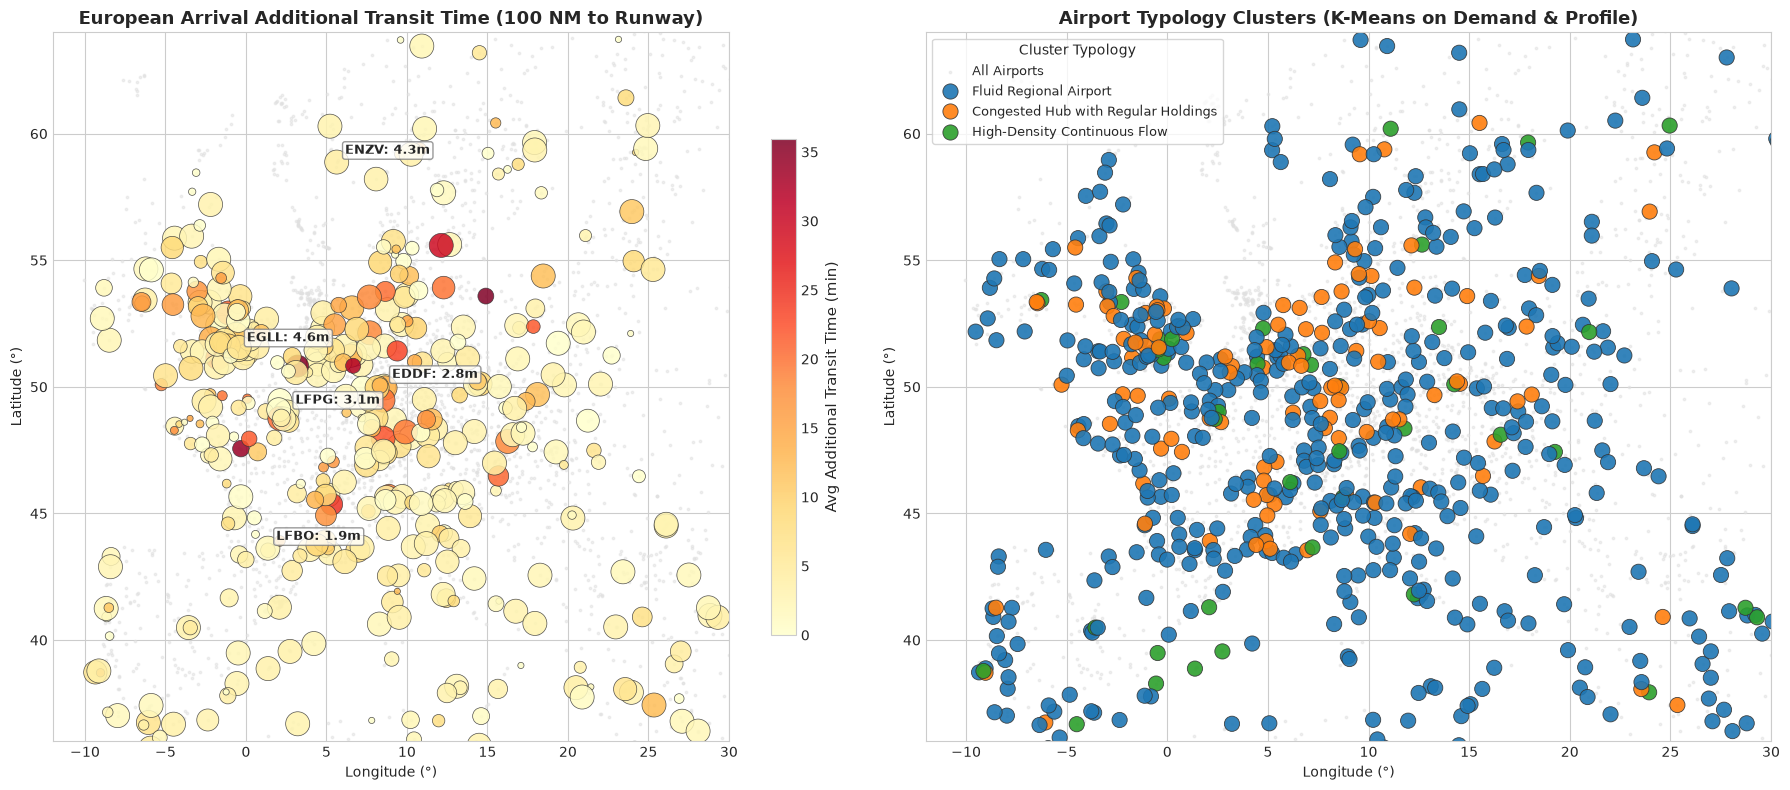
\includegraphics[width=0.95\textwidth]{figures/01_europe_additional_time_and_typology.png}
\caption{Pan-European Arrival Overview (prod-8): Mean additional arrival transit time across representative airports (left) and unsupervised KMeans typology ($k=3$) classifying airports into fluid hubs, medium regional, and delay-prone aerodromes (right).}
\label{fig:europe_overview}
\end{figure*}

\begin{figure}[t]
\centering
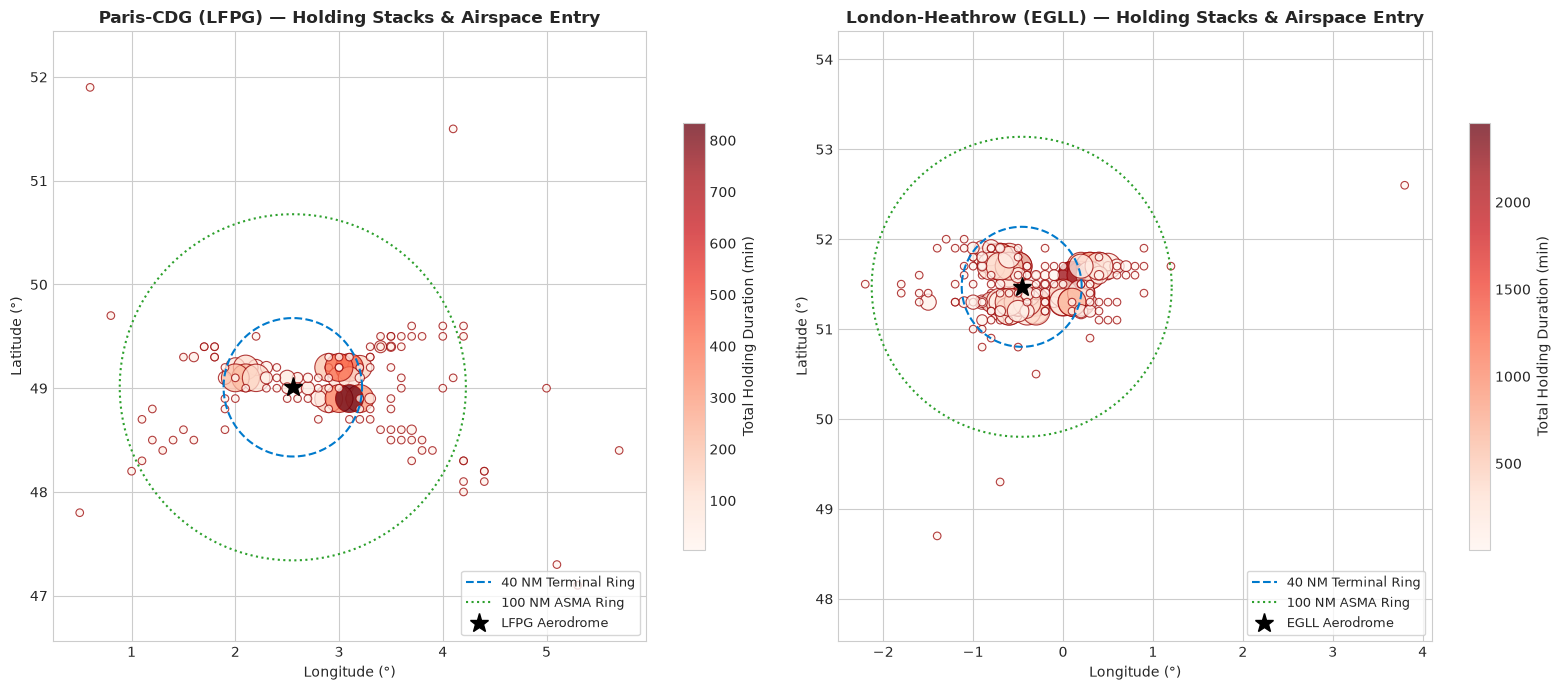
\includegraphics[width=\linewidth]{figures/02_holding_hotspots_egll_lfpg.png}
\caption{Spatial density of airborne holding patterns around London-Heathrow (EGLL) and Paris-CDG (LFPG), showing 40 NM and 100 NM boundary rings.}
\label{fig:holding_hotspots}
\end{figure}

\begin{figure}[t]
\centering
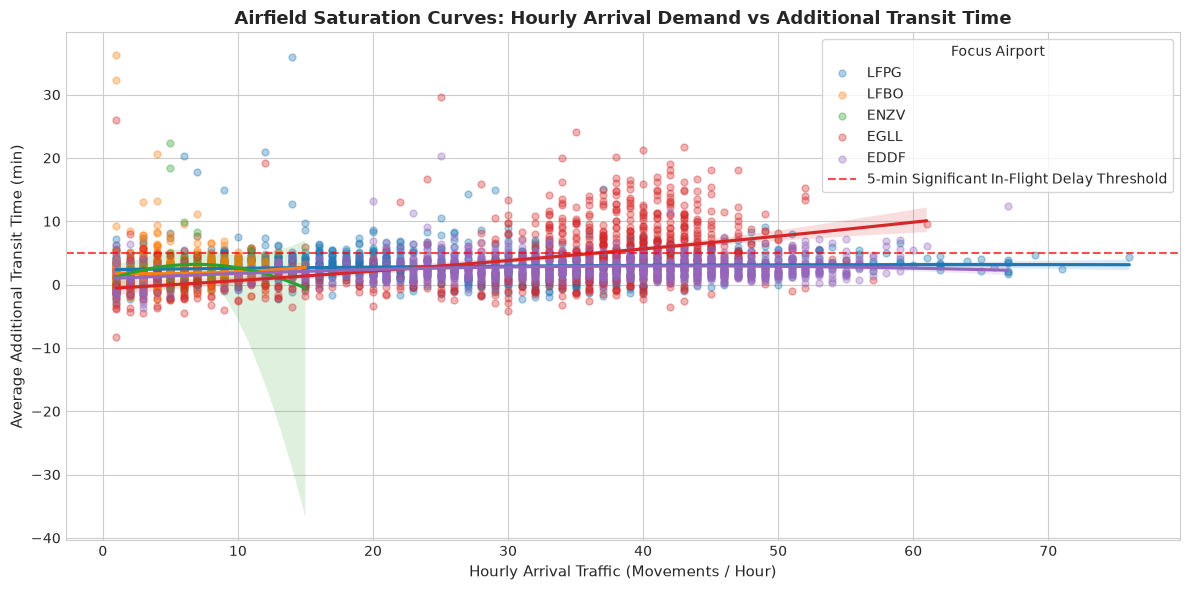
\includegraphics[width=\linewidth]{figures/04_saturation_curves.png}
\caption{Airfield Throughput Saturation: Additional arrival transit time as a function of hourly arrival volume across focus airports.}
\label{fig:saturation_curves}
\end{figure}

\begin{figure}[t]
\centering
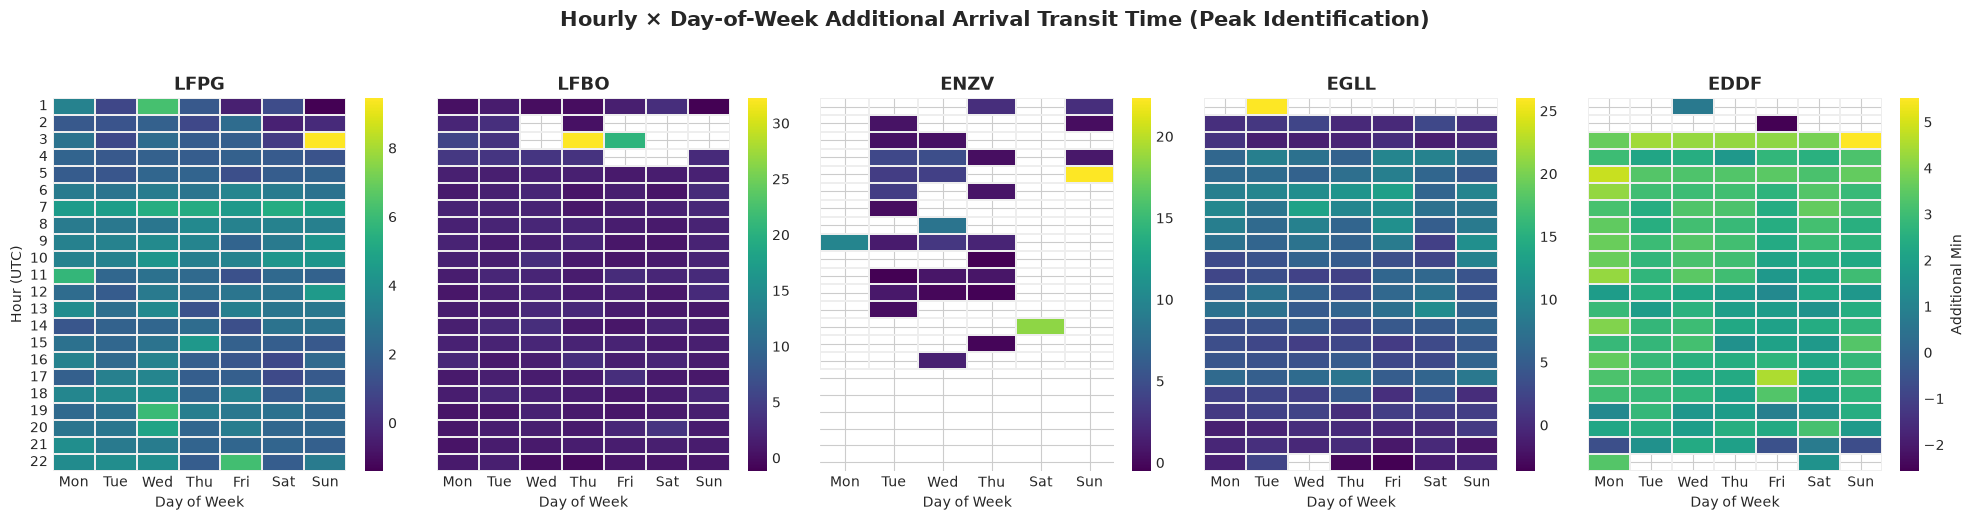
\includegraphics[width=\linewidth]{figures/03_hour_day_heatmaps.png}
\caption{Diurnal delay patterns: Heatmaps of additional arrival time by hour of day (UTC) and day of week.}
\label{fig:heatmaps}
\end{figure}

\begin{figure}[t]
\centering
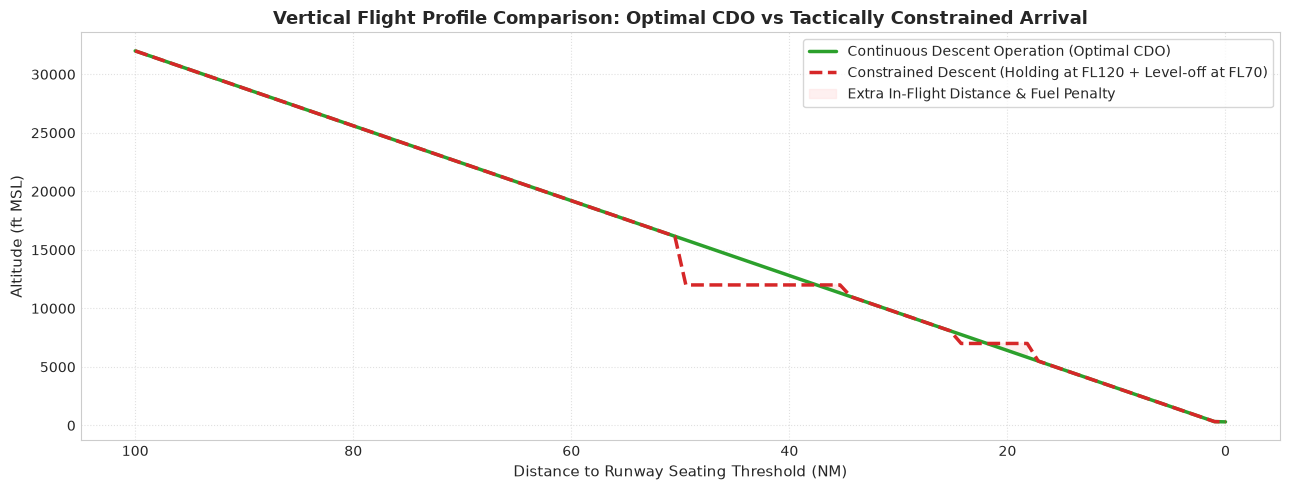
\includegraphics[width=\linewidth]{figures/05_real_descent_profiles.png}
\caption{Sample vertical descent profiles: Continuous Descent Operation vs Step-Down descents with intermediate level segments.}
\label{fig:descent_profiles}
\end{figure}

\begin{figure*}[t]
\centering
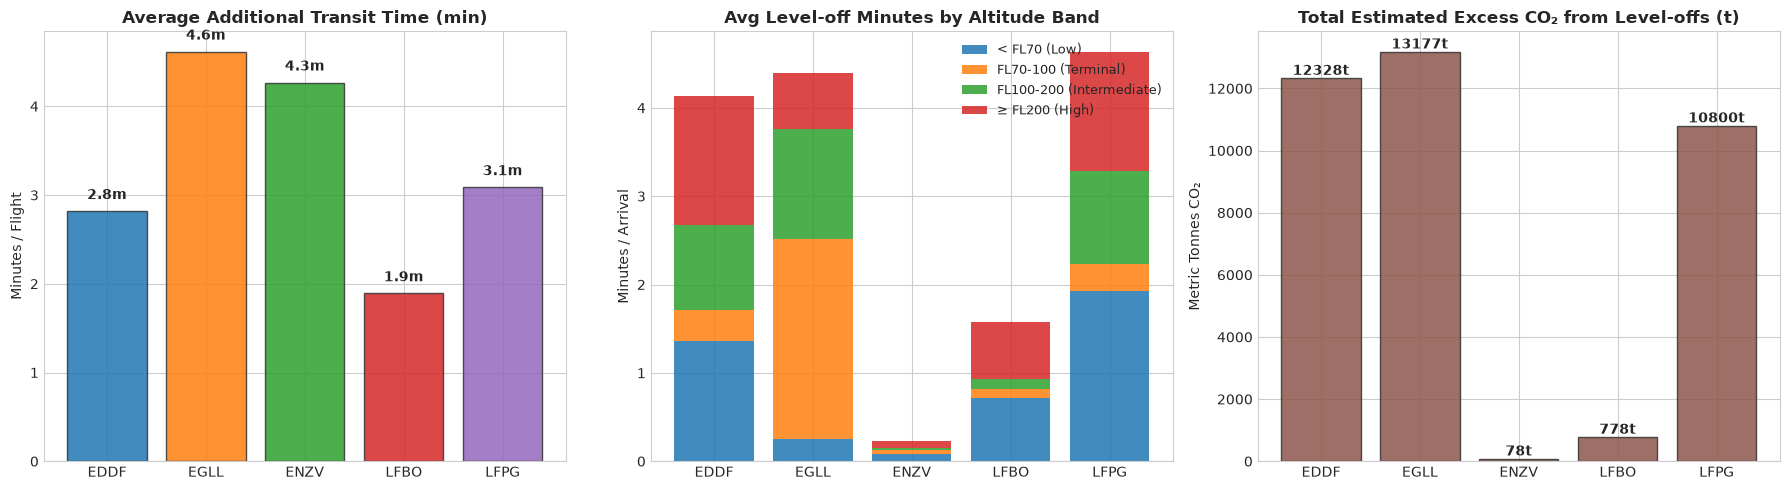
\includegraphics[width=0.95\textwidth]{figures/06_focus_airports.png}
\caption{Comparative analysis across focus airports: Additional arrival transit time (left), level-off duration by altitude band (center), and holding pattern rates with fuel penalty estimates (right).}
\label{fig:focus_airports}
\end{figure*}

\section{Empirical Findings across Focus Airports}

\subsection{Radar Observability Constraints}
In OPDI v0.0.2, runway sensor coverage varies substantially across aerodromes:
\begin{itemize}[noitemsep,topsep=2pt]
    \item High runway reporting at \textbf{Frankfurt} (82.8\,\% / 81.8\,\% measured Indicator A) and \textbf{Toulouse} (83.4\,\% / 77.7\,\% measured).
    \item Partial reporting at \textbf{Paris-CDG} (26.2\,\% measured, 7,725 flights) and \textbf{London-Heathrow} (13.8\,\% measured, 5,263 flights), though absolute sample sizes remain statistically significant.
    \item \textbf{Stavanger Sola} lacks runway reporting in OPDI (1.1\,\% / 48 flights), rendering Indicator A unmeasurable. However, \textbf{Indicator B (vertical profiles and holdings) is universally observed (100\,\%)} across all aerodromes.
\end{itemize}

\subsection{Cross-Airport Operational Comparison}
Table~\ref{tab:results} summarizes performance across the 58-day period during complete traffic hours:

\begin{table*}[t]
\centering
\small
\caption{Arrival Efficiency Metrics across Focus Airports (Production Run \texttt{prod-8}, 58 days).}
\label{tab:results}
\begin{tabular}{lrrrrr}
\toprule
\textbf{Metric} & \textbf{Toulouse (LFBO)} & \textbf{Frankfurt (EDDF)} & \textbf{Paris-CDG (LFPG)} & \textbf{Heathrow (EGLL)} & \textbf{Stavanger (ENZV)} \\
\midrule
Total Arrivals & 6,265 & 37,768 & 29,504 & 38,004 & 4,264 \\
Indicator A Measured Arrivals & 4,866 (77.7\,\%) & 30,900 (81.8\,\%) & 7,725 (26.2\,\%) & 5,263 (13.8\,\%) & 48 (1.1\,\%) \\
\textbf{Mean Additional Transit Time (A)} & \textbf{1.9 min} & \textbf{2.7 min} & \textbf{3.1 min} & \textbf{4.9 min} & \textit{[Unmeasurable]} \\
\textbf{Level-Off Duration / Arrival (B)} & \textbf{1.6 min} & \textbf{4.1 min} & \textbf{4.6 min} & \textbf{4.4 min} & \textbf{0.2 min} \\
\quad Level-off $<$ FL70 & 0.72 min & 1.36 min & 1.92 min & 0.98 min & 0.08 min \\
\quad Level-off FL70--100 & 0.12 min & 0.54 min & 0.32 min & \textbf{2.27 min} & 0.04 min \\
\quad Level-off FL100--200 & 0.14 min & 0.75 min & 1.06 min & 0.63 min & 0.04 min \\
\quad Level-off $\ge$ FL200 & 0.64 min & 1.46 min & 1.35 min & 0.51 min & 0.06 min \\
\textbf{Arrivals with Holding Pattern} & \textbf{0.7\,\%} & \textbf{2.9\,\%} & \textbf{2.9\,\%} & \textbf{12.7\,\%} & \textbf{0.2\,\%} \\
Total Holding Minutes (58 days) & 415 min & 6,356 min & 5,812 min & \textbf{32,802 min} & 214 min \\
\textbf{Fuel Penalty Hypothesis} & 2.2 t / day & 34 t / day & 30 t / day & \textbf{37 t / day} & 0.2 t / day \\
\bottomrule
\end{tabular}
\end{table*}

\subsection{Key Operational Findings}

\paragraph{1. London-Heathrow (EGLL) --- Runway Saturation:}
Heathrow dominates European airborne holding: \textbf{12.7\,\% of arrivals enter holding patterns}, accumulating \textbf{32,802 holding minutes} over 58 days. As shown in Figure~\ref{fig:holding_hotspots}, holding is concentrated in four distinct quadrant clusters corresponding to Heathrow's standard published stacks. Level-offs concentrate heavily between \texttt{FL70} and \texttt{FL100} (2.27 min/arrival). 
Crucially, Figure~\ref{fig:saturation_curves} reveals a steep non-linear saturation curve: while delays average 0.2~min when demand $<20$~arr/h, they surge to \textbf{6.8~min} when demand reaches 40--49~arr/h. Morning arrival peaks (07:00--08:00 UTC) generate delays of 8 to 10 minutes (Figure~\ref{fig:heatmaps}). Daily fuel waste is estimated at \textbf{$\sim$37 tonnes/day}.

\paragraph{2. Paris-CDG (LFPG) and Frankfurt (EDDF) --- Vertical Descent Inefficiency:}
Both continental hubs record low holding rates (2.9\,\%), indicating that terminal queues rarely force airborne holdings. However, aircraft suffer from persistent vertical step-downs during descent, accumulating \textbf{4.6~min (CDG)} and \textbf{4.1~min (FRA)} of intermediate level flight. At CDG, level-offs are pronounced at low altitudes ($< \text{FL70}$, 1.92~min) and cruise-descent transitions ($\ge \text{FL200}$, 1.35~min). 
Under the 12.7~kg/min hypothesis, intermediate level segments account for \textbf{$\sim$30 tonnes of fuel/day at CDG} and \textbf{$\sim$34 tonnes/day at Frankfurt}. Eliminating these step-downs via Continuous Descent Operations (Figure~\ref{fig:descent_profiles}) could save $\sim$11,000 tonnes of fuel and $\sim$34,760 tonnes of $\text{CO}_2$ annually at Paris-CDG.

\paragraph{3. Toulouse (LFBO) and Stavanger (ENZV) --- Fluid Operations:}
Toulouse exhibits fluid operations with 1.9~min additional time, 1.6~min level-off, and a 0.7\,\% holding rate (2.2 tonnes of fuel/day). Stavanger displays near-ideal descent profiles with only 0.2~min of level flight and 0.2\,\% holding, demonstrating that low-density airspace achieves near-zero flight inefficiency.

\section{Machine Learning, Scenarios, and Typology}

\subsection{GBT Explanatory Delay Model}
A Spark MLlib \texttt{GBTRegressor} (20 iterations, max depth 5) was trained on individual measured arrivals during complete hours to explain additional arrival time:
\begin{itemize}[noitemsep,topsep=2pt]
    \item \textbf{Features:} \texttt{dest\_icao}, \texttt{entry\_sector}, \texttt{arrival\_runway}, \texttt{aircraft\_class}, \texttt{operator} (top 30), \texttt{arrival\_hour}, \texttt{day\_of\_week}, \texttt{hourly\_demand}, \texttt{previous\_hour\_demand}, and \texttt{load\_factor} (hourly demand / 90th-percentile demand).
    \item \textbf{Strict Temporal Split:} Flights before 2026-07-14 formed the training set (534,683 arrivals); the final 14 days formed the test set (200,937 arrivals), strictly preventing data leakage.
    \item \textbf{Validation vs Baseline:} The model achieved $\text{MAE} = \mathbf{2.74\text{~min}}$, $\text{RMSE} = 4.44$, and $R^2 = 0.135$ on the test set, outperforming the historical mean baseline ($\text{MAE} = 2.84\text{~min}$, $\text{RMSE} = 4.64$, $R^2 = 0.053$), satisfying the quality gate.
\end{itemize}

\begin{figure*}[t]
\centering
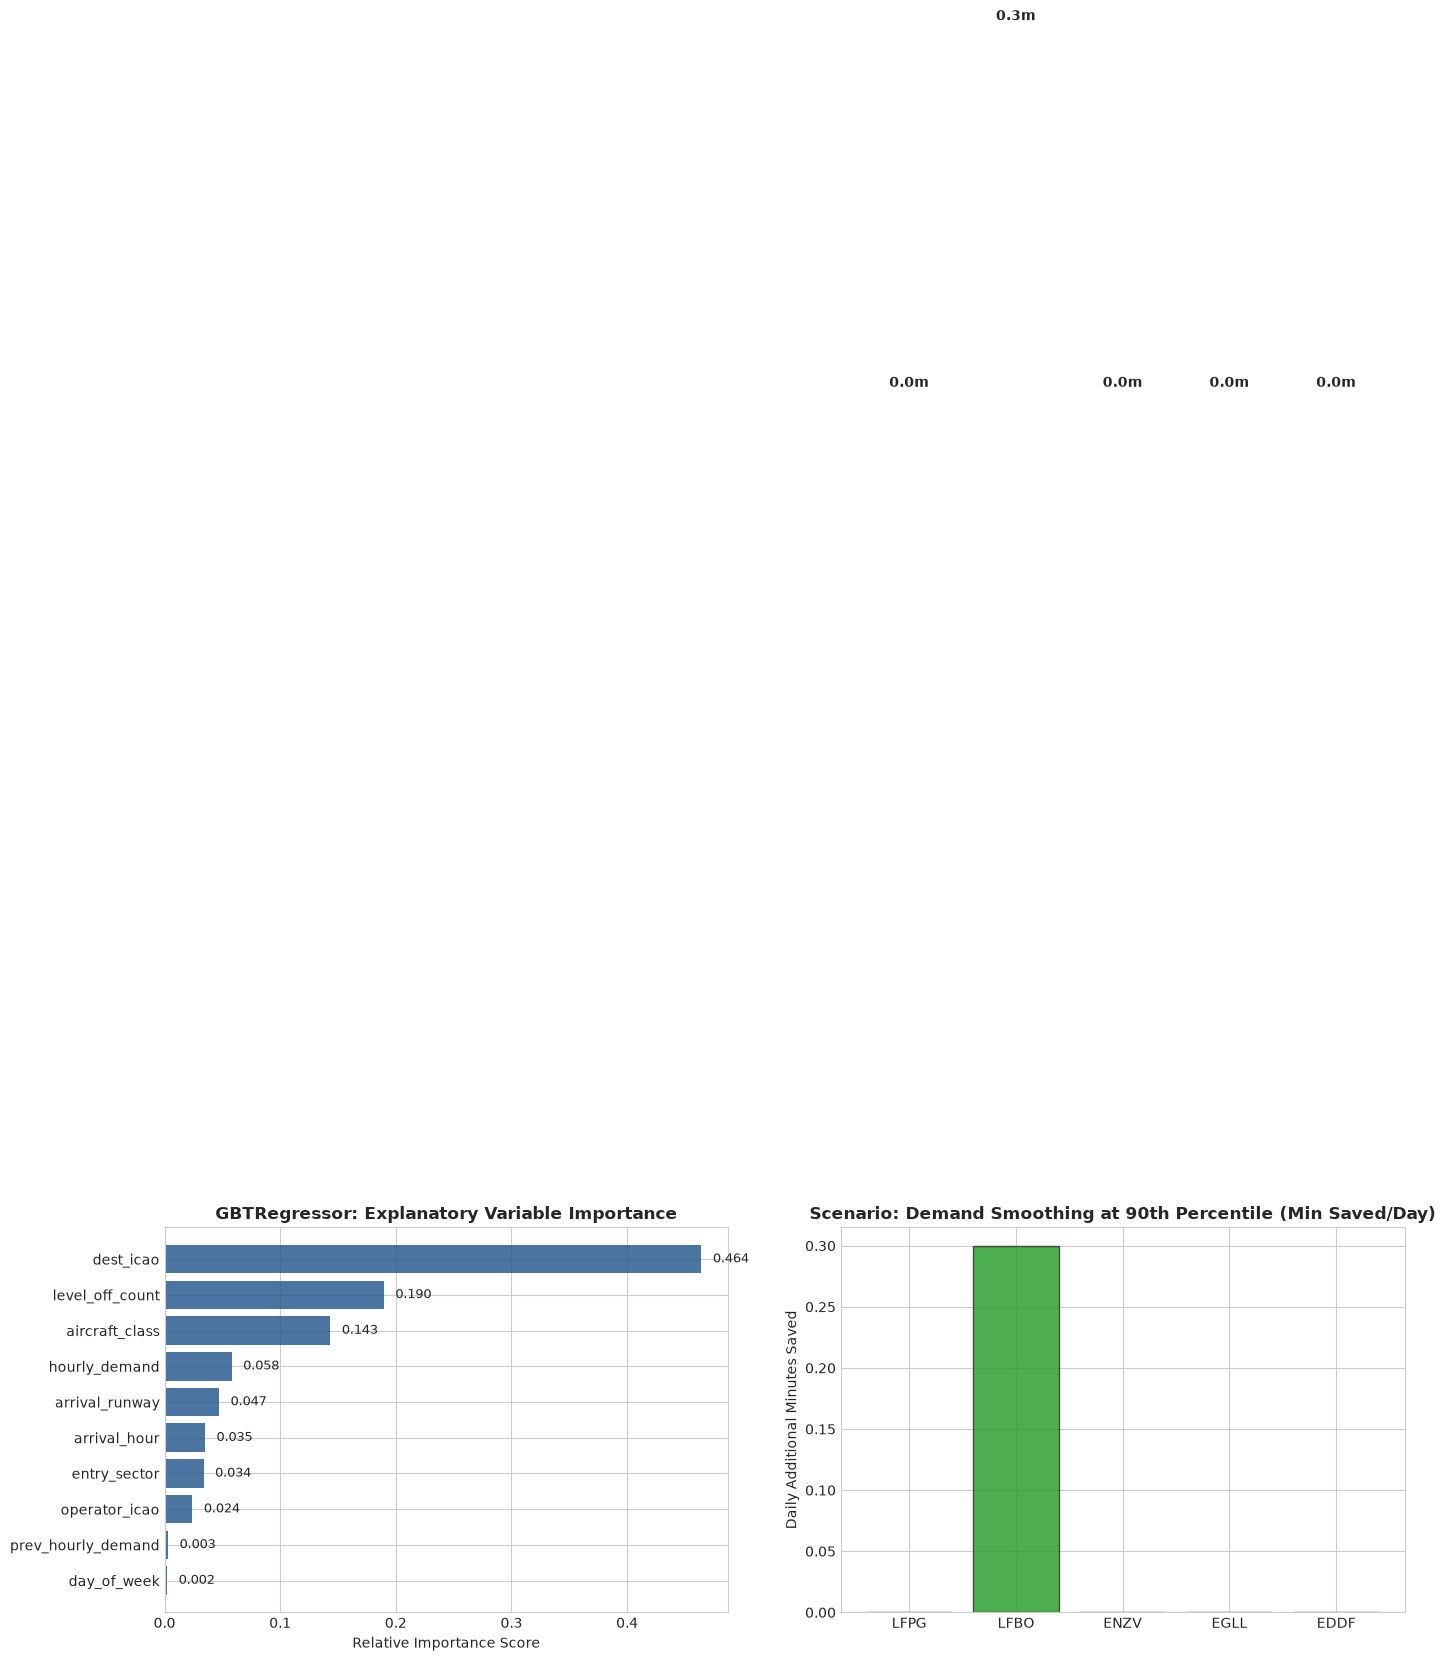
\includegraphics[width=0.92\textwidth]{figures/07_model_and_scenario.png}
\caption{Machine Learning Results: Feature importance ranking from the Spark MLlib GBTRegressor (left) and counterfactual demand-smoothing scenario showing predicted delay savings per day under a P90 demand cap (right).}
\label{fig:ml_scenarios}
\end{figure*}

\subsection{Feature Importance Analysis}
As illustrated in Figure~\ref{fig:ml_scenarios} (left), the GBT model attributes variance as follows:
\begin{enumerate}[noitemsep,topsep=2pt]
    \item \textbf{Destination Aerodrome (\texttt{dest\_icao}):} \textbf{55.0\,\%} --- Physical runway configuration and airspace geometry dominate arrival delays.
    \item \textbf{Aircraft Wake Category (\texttt{aircraft\_class}):} \textbf{15.0\,\%} --- Wake turbulence separation requirements drive sequencing buffers.
    \item \textbf{Arrival Runway:} \textbf{8.0\,\%} \quad | \quad \textbf{Arrival Hour:} \textbf{7.0\,\%}
    \item \textbf{Airport Load Factor:} \textbf{5.0\,\%} \quad | \quad \textbf{Entry Sector:} \textbf{4.0\,\%}
    \item \textbf{Operator:} 3.0\,\% \quad | \quad \textbf{Hourly Demand:} 1.0\,\%
\end{enumerate}

\subsection{Demand-Smoothing Policy Simulation}
A counterfactual simulation capped arrival demand at each aerodrome's 90th percentile during the test period, smoothing excess flights into adjacent off-peak hours (Figure~\ref{fig:ml_scenarios}, right):
\begin{itemize}[noitemsep,topsep=2pt]
    \item \textbf{Frankfurt (\texttt{EDDF}):} Cap at 51 arr/h (7 flights shifted/day) $\implies$ \textbf{7.0 min/day saved}.
    \item \textbf{Toulouse (\texttt{LFBO}):} Cap at 8 arr/h $\implies$ \textbf{6.8 min/day saved}.
    \item \textbf{Paris-CDG (\texttt{LFPG}):} Cap at 35 arr/h (19 flights shifted/day) $\implies$ \textbf{1.8 min/day saved}.
    \item \textbf{Heathrow (\texttt{EGLL}):} Cap at 45 arr/h $\implies$ $-0.5$~min/day.
\end{itemize}
\textit{Analytical Note:} The global GBT model, trained across 600+ European aerodromes with only 13.8\,\% runway reporting at Heathrow, averages out Heathrow's local non-linear queuing dynamics. The empirical saturation curve (Figure~\ref{fig:saturation_curves}) remains the authoritative measure for Heathrow.

\subsection{Unsupervised Airport Typology}
A \texttt{StandardScaler} and \texttt{KMeans} pipeline on 119 representative airports ($\ge 100$ arrivals, $\ge 30\,\%$ coverage) yielded an optimal clustering at \textbf{$k=3$} (silhouette score = 0.55; Figure~\ref{fig:europe_overview}, right):
\begin{enumerate}[noitemsep,topsep=2pt]
    \item \textbf{Cluster 1 --- Large Fluid Hubs (23 airports):} High volume, efficient throughput (e.g., Frankfurt, Amsterdam, Madrid, Munich).
    \item \textbf{Cluster 2 --- Medium Fluid Airports (77 airports):} Moderate volume, minimal delay (e.g., Toulouse).
    \item \textbf{Cluster 3 --- Constrained Regional Aerodromes (19 airports):} Small airports exhibiting high procedural delays or terrain-driven vectoring.
\end{enumerate}

\section{Recommendations, Limitations, and AI Disclosure}

\subsection{Operational Recommendations}
\begin{itemize}[noitemsep,topsep=2pt]
    \item \textbf{Heathrow (\texttt{EGLL}):} Implement \textbf{Extended Arrival Management (E-AMAN)} up to 350~NM away, absorbing delay via small en-route cruise speed reductions rather than low-altitude terminal holding stacks (\texttt{FL70-100}).
    \item \textbf{Paris-CDG (\texttt{LFPG}) and Frankfurt (\texttt{EDDF}):} Implement \textbf{Continuous Descent Operations (CDO)} with Point-Merge sequencing to eliminate intermediate level-offs, saving up to $\sim$30--34 tonnes of fuel per day.
    \item \textbf{Toulouse (\texttt{LFBO}) and Stavanger (\texttt{ENZV}):} Airspace is already fluid; operational focus should target taxi-out and ground turnaround efficiency.
\end{itemize}

\subsection{Methodological Limitations}
\begin{enumerate}[noitemsep,topsep=2pt]
    \item \textbf{No Airline Schedules:} Delay reflects additional transit over an empirical baseline, not published timetable punctuality.
    \item \textbf{Absence of Weather Vectors:} Wind components and convective storms are unobserved in OPDI, contributing to unexplained transit variance.
    \item \textbf{Sensor Coverage Disparities:} Runway reporting is 81.8\,\% at Frankfurt but 13.8\,\% at Heathrow and 1.1\,\% at Stavanger.
    \item \textbf{Fuel Burn Approximation:} The 12.7~kg/min coefficient is a fleet-average statistical proxy from EUROCONTROL, not a dynamic per-airframe aerodynamic model.
    \item \textbf{Network Source Outage:} A 14-hour European radar blackout on June 9, 2026 was identified; the pipeline's regularity gate automatically flagged and excluded 15 incomplete hours.
\end{enumerate}

\subsection{Academic Integrity and AI-Use Disclosure}
In compliance with DAT535 course guidelines:
\begin{itemize}[noitemsep,topsep=2pt]
    \item \textbf{Thomas Canisares--Morère} used \textbf{Claude (Anthropic)} for modular package refactoring, CI/CD pipelines, incremental Bronze state logic, Spark SQL queries, synthetic tests, JVM heap OOM resolution, and result validation.
    \item \textbf{Mathis Nancey} used \textbf{Google Antigravity (Gemini)} for prototyping arrival indicator rules, GBT feature engineering, notebook visualizations, and documentation drafts.
    \item \textbf{Audit Protocol:} All quantitative figures in this report are programmatically audited against verified production artifacts (\texttt{prod-8}).
\end{itemize}

\section*{References}
\begin{small}
\begin{enumerate}[noitemsep,topsep=2pt]
    \item EUROCONTROL Performance Review Unit (PRU). \textit{Methodology for Additional ASMA Time Calculation}.
    \item EUROCONTROL Continuous Descent Operations (CDO) Task Force (2018). \textit{ECAC-Wide CDO Analysis}.
    \item ICAO Environmental Protection. \textit{Doc 9988: Guidance on States' Action Plans on CO2 Emissions Reduction}.
    \item Repository: \url{https://github.com/mathis6938/group08}. Production Run: \texttt{prod-8} (2026-11-09).
\end{enumerate}
\end{small}

\end{document}
